% Thanks to Seth Johnson (sethrj@umich.edu) for publishing his ans template

%%%%%%%%%%%%%%%%%%%%%%%%%%%%%%%%%%%%%%%%%%%%%%%%%%%%%%%%%%%%%%%%%%%%%%%%%%%%%%%%
\documentclass{anstrans}
\bibliographystyle{ans}

%%%%%%%%% title %%%%%%%%%
\title{An Agent-Based Framework for Fuel Cycle Simulation with Recycling}
\author{Matthew J.~Gidden, Paul P.H.~Wilson, Kathryn D.~Huff, Robert W.~Carlsen}
\institute{Department of Nuclear Engineering \& Engineering Physics, University of Wisconsin - Madison, Madison, WI, 53703}
\email{gidden@wisc.edu}
\date{2013/01/14}

%%%%%% preamble %%%%%%%%%%

%%%%%%%%%%%%%%%%%%%%%%%%%%%%%%%%%%%
\usepackage{times} % fancier looking type
\usepackage{graphicx}
\usepackage{microtype} % if using PDF
\usepackage{amsmath} % for optimization equations
\usepackage{booktabs}

%% Custom Commands from Katy Huff
\newcommand{\Cyclus}{\textsc{Cyclus} }
\newcommand{\nucl}[2]{
\ensuremath{^{#1}}\mbox{#2}
}

%% Packages added by Matt Gidden
\usepackage{moreverb} % for verbatim snippets of code
\usepackage{fancyvrb}
\usepackage{tabularx} % for tables with line breaks
\usepackage{calc} % allows for arithmetic on latex variables

%% Custom commands added by Matt Gidden
\newcommand{\Cyclopts}{\textsc{Cyclopts} }


%%%%%%%%%%%%%%%%%%%%%%%%%%%%%%%%%%%%%%%%%%%%%%%%
\begin{document}

%%%%%% abstract %%%%%%%%%%
\textit
{ Simulation of the nuclear fuel cycle is an established field with multiple
  players.  Prior development work has utilized techniques such as system
  dynamics to provide a solution structure for the matching of supply and demand
  in these simulations. In general, however, simulation infrastructure
  development has occured in relatively closed circles, each effort having
  unique considerations as to the cases which are desired to be
  modeled. Accordingly, individual simulators tend to have their design
  decisions driven by specific use cases. Presented in this work is a proposed
  supply and demand matching algorithm that leverages the techniques of the
  well-studied field of mathematical programming. A generic approach is achieved
  by treating facilities as individual entities and actors in the supply-demand
  market which denote preferences amongst commodities. Using such a framework
  allows for varying levels of interaction fidelity, ranging from low-fidelity,
  quick solutions to high-fidelity solutions that model individual transactions
  (e.g. at the fuel-assembly level). The power of the technique is that it allows
  such flexibility while still treating the problem in a generic manner,
  encapsulating simulation engine design decisions in such a way that future
  simulation requirements can be relatively easily added when needed.  }


%%%%%% intro %%%%%%%%%%
\section{Introduction}\label{sec:intro}

\begin{frame}[ctb!]
  \frametitle{\Cyclus}
  
\end{frame}

\begin{frame}[ctb!]
  \frametitle{Motivating Question}
  
  \begin{block}{Dynamic Resource Exchange}
    If facilities are treated as individual black boxes and connections between
    facilities are determined dynamically, how does one match suppliers with
    demanders considering supply constraints and, supply response to
    quality-based demands, and issues of fungibility?
  \end{block}

\end{frame}


%%%%%% background %%%%%%%%%%
\section{Background}\label{sec:background}
\subsection{Fuel Cycle Simulators}

Previous implementations of fuel cycle simulators have varied both in
methodology and distribution platform. The general purpose of all simulators is
to model the flow of material around the fuel cycle in order to determine the
viability of various proposed fuel cycles and their relative
performance \textit{vis-a-vis} a variety of metrics including resource
utilization, costs, and proliferation resistance. However, there are a few key
choices that have been historically made by all simulation developers,
including: what program or language to use, how to determine the flow of
material when there are competing sources or sinks for that material, how to
determine which facilities to build and when to build them, and at what level of
fidelity simulation physics should be modeled (e.g., should material decay or
should it not). One could describe these are the major design choices for
simulation development teams to assess, and in general approaches are taken
which span the gamut from the computationally ``easy'' to the computationally
``complex'' and the spectrum of almost full user-control to more substantial use
of automated decision making.



\subsection{Agent Based Supply Chain Simulation}

There are a number of agent-based supply chain frameworks and implementations
available in the literature with varying levels of accessibility due to
proprietary
considerations \cite{swaminathan_modeling_1998,julka_agent-based_2002,van_der_zee_modeling_2005,chatfield_multi-formalism_2007}.
However, the nuclear fuel cycle presents a few unique characteristics not
explicitly treated in the literature. Perhaps the most difficult consideration
we have identified is the need to specify target fuel recipes and match
suppliers and consumers based on the requested recipe, i.e.  there are both
quantity and quality constraints placed on a requested commodity. An additional
difficulty arises with the enforcement of regional-boundary constraints
(e.g. prohibiting HEU trade between regions) and inter-enterprise
preferences. We propose to tackle both issues via a comprehensive supply/demand
matching mechanism.

We propose using a supply/demand matching algorithm that is comprised 
of three main procedures: request-for-bids, preference assignment, 
and resolution. The request-for-bids step signals the producers of 
various commodities of the demand and material specification for 
those commodities. The preference assignment step allows the customers
to analyze each bid in order to assign a preference. The managers of 
these customers (be they at the region or enterprise level) are 
allowed to affect the decision making process at this point in order 
to inform the preferences of the customers covered by their policy 
space. The resolution step takes the as input the bids and 
preferences and outputs the material flows for the given time step.\cite{cyclus2012}

\subsection{Mathematical Programming}


%%%%%% methodology %%%%%%%%%%
\section{Methodology}\label{sec:methodology}


\begin{frame}[ctb!]
  \frametitle{\Cyclus}
  
\end{frame}

\begin{frame}[ctb!]
  \frametitle{Motivating Question}
  
  \begin{block}{Dynamic Resource Exchange}
    If facilities are treated as individual black boxes and connections between
    facilities are determined dynamically, how does one match suppliers with
    demanders considering supply constraints and, supply response to
    quality-based demands, and issues of fungibility?
  \end{block}

\end{frame}


\subsection{Agent Interaction in \Cyclus}\label{sec:agent-interaction}
This sections describes the simulation interaction between agents. Of the
research directions presented in this chapter, it is definitely the most
malleable. Deciding how a simulation is structured from an interactions
standpoint is a delicate balance of known necessity and perceived future
needs. There are basic decisions to make: do you want a system with discrete
material transfers or continuous material flows? Discrete transfers more closely
match reality and may provide insights in that regard, however the require more
of their modeling apparatus due to messaging needs and other structures. More
complex decisions include how one wants to determine connections between
facilities. Do we assign supplier-consumer pairs to facilities? Do we allow them
to change? Should the facility make such a decision? Should that decision be
affected by any other entities? Guerin's comment in \S\ref{sec:intro-benchmarks}
stems from this ``freedom''. These simulation-engine decisions comprise the
art-related portion of fuel cycle simulation. The goal is to make these
decisions in as informed a way as possible from our domain-level knowledge with
respect to our known and perceived requirements. In general, we try to minimize
the sheer number of choices we make in this regard, instead relying on well
known and well documented practices of computer scientists and systems
engineers.

\Cyclus has an additional goal in that we wish our core simulation
infrastructure to be as flexible as possible. Given a few basic tenets of agent
interaction, other developers should be able to create a new agent to ``plug
in'' to the simulation. Accordingly, we must define a minimal set of behaviors
to sufficiently inform the simulation infrastructure to run the simulation. This
freedom allows us to run the simulation program and attach agents at run time,
effectively separating the simulation engine's functionality from the agents in
the simulation. From an ecosystem point of view, being an open source code and
having such capability allows expansion of the user and developer base into
areas and institutions concerned with security and privacy. Furthermore,
developers could participate both privately and publicly, e.g. adding general
capability to the \Cyclus core that is needed for some functionality without
specifying the internals. Such a community paradigm is shown in Figure
\ref{fig:community}.

\begin{figure}[htbp!]
  \begin{center}
    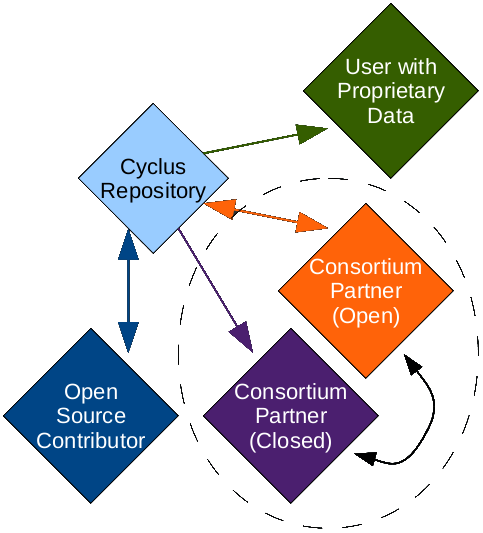
\includegraphics[height=8cm]{./parts/method/community.png}
  \end{center}
  \caption{The Cyclus Participation Paradigm} 
  \label{fig:community}
\end{figure}

This open-source ecosystem further provides incentive to develop the agent-based
simulation architecture. Other developers can concentrate their efforts on
individual agent interaction, effectively encapsulating developer requirements
for learning and interacting with the various simulation systems. Having decided
upon agent-based interactions, one must determine a way to govern these
interactions. We want to minimize agent dependency due to our above discussion,
so using preference-based network flow formulations provide us with a viable
solution technique that provides a consistent interface. The remainder of this
section describes how that market resolution interface is informed by the
agents. Basic agent simulation interaction, such as entering and leaving the
simulation are also described.

\subsection{Supply/Demand Parameters}

The resolution of supply and demand at any given time step is the result of the
mathematical program techniques described in \S\ref{sec:gfctp}; however, there
are simulation-engine details that must be described in order to set up that
problem. The proposed resolution mechanism occurs in nominally three steps. The
agent interactions include consumers and producers of a set of commodities and
progresses is steps or ``phases''. The terminology of this ``phase space'' is
taken from previous supply chain agent-based modeling
work \cite{julka_agent-based_2002}.

The first phase allows consumers of commodities to denote both the quantity of a
commodity they need to consume as well as the target isotopics, or
quality. Because the action of posting is technically telling possible providers
what type of product or service is required by a facility, this phase is termed
the ``Request for Bids Phase''. This action is considered a ``posting'' of
demand to the market exchange. Consumers are allowed to ``over-post'', i.e.,
request more quantity than they can actually consume as long as a corresponding
capacity constraint accompanies this posting. Further, consumers are allowed to
post demand for multiple commodities that may serve to meet the same combine
capacity. For example, consider an LWR that can be filled with MOX or UOX. It
can post a demand for both, but must define a preference over the set of
possible commodities it can consume. Another example is that of an advanced fuel
fabrication facility, i.e., one that fabricates fuel partially from separated
material that has already passed through a reactor. Such a facility can choose
to fill the remaining space in a certain assembly with various types of fertile
material, including depleted uranium from enrichment or reprocessed uranium from
separations. Accordingly, it could demand both commodities as long as it
provides a corresponding constraint with respect to total consumption. At the
end of the posting phase, the market exchange will have a set of consumption
portfolio for each consumer. Each consumption portfolio may be constituted by
multiple consumption requests, and each may have a detailed isotopic quality
defined; however, there must be a cardinal preference over the requests in the
portfolio and an overall capacity for the portfolio.

The second phase allows suppliers to ``respond'' to the set of consumption
portfolios. Each portfolio is comprised of requests for some set of
commodities. Accordingly, for each request, suppliers of that commodity denote
production capacities and an isotopic profile of the commodity they can
provide. This isotopic profile is part of a heuristic mechanism to assign more
fine-grained preferences among suppliers and consumers. Suppliers are allowed to
offer the null set of isotopics as their profile, effectively providing no
information. A supplier may have its production be constrained by more than one
parameter. For example, a processing facility may have both a throughput
constraint (i.e., it can only process material at a certain rate) and an
inventory constraint (i.e., it can only hold some total material). Further, the
facility could have a constraint on the quality of material to be processed,
e.g., it may be able to handle a maximum radiotoxicity for any given time step
which is a function of both the quantity of material is processes but also the
isotopic content of that material. The formulation provided in \S\ref{sec:gfctp}
allows for multiple of such constraints as long as they are linear functions of
the demanded commodity quantity. This phase is termed the ``Response to Request
for Bids Phase'', and at its completion the possible connections between supplier and
producer facilities, i.e., the arcs in the graph of it transportation problem,
have been established with specific capacity constraints defined both by the
quantity of commodities that will traverse the arcs but also by the quality.

The third phase of setting the exchange market parameters involves setting
preference values for each supplier-consumer arc, thus this phase is termed the
``Preference Assignment Phase''. These values will eventually be converted to
costs in order to solve variant of the multi-commodity transportation problem,
in which the inversion technique itself is a simulation design decision. In any
case, this phase begins with the consumers. Each consumer has already assigned
preferences as a function of commodity amongst requests in its portfolio. The
consumer is now allowed to inform the solver as to preferences amongst the
responses to each request in each portfolio. These delineations will nominally
be made as a function of the quality of the material in the big response. For
example, a reactor may request MOX and UOX. It may get two responses to its
request for MOX, each with different isotopic profiles of the MOX that can be
provided. It can then assign preference values over this set of potential MOX
providers. Another prime example is in the case of repositories. A repository
may have a defined preference of material to accept based upon its heat load or
radiotoxicity, both of which are functions of the quality, or isotopics, of a
material. In certain simulators, limits on fuel entering a repository are
imposed based upon the amount of time that has elapsed since the fuel has exited
a reactor. It is in this phase that the \Cyclus engine would allow such
capability. The time constraint is, in actuality, a constraint on heat load or
radiotoxicity (one must let enough of the fission products decay). A repository
could analyze possible input fuel isotopics and set the arc preference of any
that violate a given rule to 0, effectively eliminating that arc. Once
facilities have completed their preference assignments, their managers are able
to permute them based on institutional or regional factors, explained below.

\subsection{Facilities}

Facilities in \Cyclus are abstracted to either consumers or suppliers of
commodities, and some may be both. Supplier agents are provided agency by being
able to communicate to the market-resolution mechanism a variety of production
capacity constraints in phase two of the solution setup. Consumer agents are
provided agency by being able to assign preferences among possible suppliers
based on the supplier's quality of product. Because this agency is encapsulated
for each agent, it is possible to define strategies that can be attached or
detached to the agents at run-time. Such strategies are an example of the
Strategy design pattern \cite{vlissides_design_1995}.

\subsection{Institutions}

Institutions in \Cyclus manage a set of facilities. They are tasked with the
actual instantiation of specific facilities, e.g. it is the institutions job to
manage which facilities are commissioned and decommissioned at the appropriate
times. The goal of including a notion of institutions is to allow an increased
level of detail when investigating regional-specific scenarios. For example,
there exist multi-national enterprises, such as AREVA, that operate fuel cycle
facilities in a variety of countries, or regions. Furthermore, there are
international governmental organizations, such as the IAEA, which operate fuel
cycle facilities that service other facilities in a variety of regions. A fuel
bank is an example of such a facility. Accordingly, institutions in \Cyclus are
able to augment the preferences of supplier-consumer pairs that have been
established in order to simulate a mutual preference to trade material within an
institution. Of course, situations arise in real life where an institution has
the capability to service its own facilities, but choose to use an outside
provider because of either cost or time constraints. Such a situation is allowed
in this framework as well. It is not clear how such a relationship should be
instantiated and to what degree institutions should be allowed to affect their
managed facilities' preferences. This issue lies squarely in the realm of
simulation design decisions, part of the ``art'' of simulation. Accordingly,
through the course of research, the possible design space will be analyzed in
order to determine best practices for this type of design.

\subsection{Regions}

Regions in \Cyclus are concerned with meeting certain requirements, e.g. power
capacity, fuel cycle service capacity, etc. The notion of which facilities will
meet this capacity is abstracted away from the region into the set of
institutions that operate in that region. In other words, in the case of nuclear
power capacity, a region knows that it needs additional reactors to be built,
but leaves the building of those reactors to the institutions that operate in
the region. However, given information regarding the possible reactors that can
be built, the region can order which reactors should be built by which
institutions. Again, the idea here is to abstract the management of facilities
away from the decision of which facilities to build. It is important to note
here that this abstraction allows for different deployment algorithms to be
tested and exchanged in the \Cyclus framework without necessitating changes to
the simulation engine, as is the case with other simulators described
in \S\ref{sec:simulators} and is consistent with the types of simulation design
decisions described in \S\ref{sec:simulators-overview}. Regions are further
provided agency by their ability to affect preferences between supplier-consumer
facility pairs in the third phase of the market resolution algorithm. The
ability to perturb arc preferences between a given supplier and a given consumer
allows fuel cycle simulation developers to model relatively complex interactions
at a regional level. Examples of such interactions include the notion of
tariffs, i.e., a region may prefer that facilities that can trade within its
borders to so. Further, one could model the affect of sanctions, i.e., a region
may not allow trade between facilities within its borders and another specified
region. Finally, constraints can be applied on the quality of material that may
occur in a transaction. For example, a region could scan the set of possible
material leaving its borders via supplier transactions. It could then affect the
preference of transactions that violate some principle, such as ``no MOX can
leave my boundaries''. These principles can even exist on a spectrum, e.g. ``no
MOX with a certain content can leave my boundaries'', or be region-specific,
e.g. ``no MOX can leave my boundaries that will go to some specified
region''. Again, these policies are prime examples of strategies that can be
implemented via the Strategy pattern.


\subsection{The Generic Fuel Cycle Transportation Problem}\label{sec:gfctp}

\subsubsection{Formulation}

In formulating the Generic Fuel Cycle Transportation Problem (GFCTP), note that
the ``players'' in the set of commodity ``markets'' are the individual
facilities involved in the simulation, i.e., the reactors, fabrication
facilities, repositories, etc. In strict mathematical programming parlance, the
GFCTP can be described as a Mixed-Integer, Multicommodity Transportation Problem
(MTP) with Side Constraints. Accordingly are a number of departures from the
classical MTP that was described in \S\ref{sec:MCTP}.

To begin, the multicommodity aspect of the problem is not manifest on arc
capacities. Instead, facility demand constraints incorporate a set of
satisfactory commodities. For example, a reactor may be able to accept UOX or
MOX fuel, but has a demand for total fuel. Additionally, supplier facilities may
have a set of constraints on their ability to supply a given commodity and they
may not be able to directly express those constraints with the unit of the
commodity market, i.e., kilograms. Take for example an enrichment facility. Such
a facility has nominally two constraints: SWU capacity and natural uranium
capacity. The former constraint is temporal, i.e., it is a processing
constraint. The latter constraint is an inventory constraint. However, both are
necessary to fully define the problem. Furthermore, let us note that the output
of this facility is kilograms of enriched uranium. Accordingly, the above
capacities must be translated into this output. Finally, realism is introduced
through integer variables. For a number of facilities, especially reactors, it
may not be realistic for a given fuel order to be split amongst a variety of
suppliers. The realm of integer programming techniques allow us to introduced
binary variables to enforce this reality constraint.

It should be noted that the addition of integer variables changes both the
complexity of the formulation and the complexity of the solution technique. Such
a change requires a Mixed Integer-Linear Program (MILP) formulation and solution
via the branch-and-bound method (see \S\ref{sec:bnb}) which solves NP-Hard
combinatorial optimization problems whereas the Linear Program (LP) version
requires the transportation simplex method (see \S\ref{sec:trans-simplex})
which is solvable in polynomial time.  Accordingly, I describe the full
formulation in two parts below: \S\ref{sec:GFCTP-LP} describes the linear
program formulation with side constraints which I will denote GFCTP-LP
and \S\ref{sec:GFCTP-E} describes the MILP formulation with side constraints
which I will denote GFCTP-E (E stands for ``exclusive'', i.e., integer variables
denote an exclusive selection of consumers and/or producers).

\subsubsection{Linear Program with Side Constraints Formulation}\label{sec:GFCTP-LP}


The Generic Fuel Cycle Transportation Problem with Side Constraints (GFCTP-LP)
describes a multi-commodity setting in which demand can be met by multiple
commodities. Consumers denote a cost preference over the possible commodities
they consume and a demand for the set of commodities that must be met. Suppliers
denote one or more production capacities for a given commodity which serve as
the set of supply capacities analogous to the normal MCTP
(see \S\ref{sec:MCTP}). The GFCTP-LP formulation is as follows:

%%% 
\begin{subequations}\label{eqs:GFCTP-LP}
  \begin{align}
    %%
    \min_{z} \:\: & 
    z = \sum_{h \in H}\sum_{i \in I}\sum_{j \in J}c_{i,j}^{h} x_{i,j}^{h} 
    & \label{eqs:GFCTP-LP_obj} \\
    %%
    \text{s.t.} \:\: &
    \sum_{j \in J}\beta_{i,k}(q_{j}^{h}) x_{i,j}^{h} \leq s_{i,k} 
    &
    \: \forall \: k \in K_{i}^{h},  
    \forall \: i \in I, \forall \: h \in H \label{eqs:GFCTP-LP_sup} \\
    %%
    &
    \sum_{i \in I}\sum_{h \in H_{j}} x_{i,j}^{h} \geq d_{j}(H_{j}) 
    & 
    \forall \: j \in J \label{eqs:GFCTP-LP_dem} \\
    %%
    &
    x_{i,j} \geq 0
    &
    \forall \: x \in X \label{eqs:GFCTP-LP_x}
    %%
  \end{align}
\end{subequations}
%%% 

The sets and variables involved are described in Tables \ref{tbl:GFCTP-LP-sets}
and \ref{tbl:GFCTP-LP-vars}. Note that $H_{j}$ is a subset of the commodities:

\begin{equation}
  H_{j} \subseteq H \: \forall \: j \in J
\end{equation}

%%% 
\begin{table} [h!]
\centering
\begin{tabularx}{\columnwidth-10pt}{|c|X|} % line wraps second column if too long
\hline
Set         & Description \\
\hline
$H$         & all commodities  \\
$I$         & all producers  \\
$J$         & all consumers  \\
$X$         & the feasible set of flows between producers and consumers  \\
$K_{i}^{h}$  & the set of constraining capacities for 
            producer $i$ of commodity $h$  \\
$H_{j}$     & the set of satisfying commodities for consumer $j$  \\
\hline
\end{tabularx}
\caption{Sets Appearing in the GFCTP-LP Formulation}
\label{tbl:GFCTP-LP-sets}
\end{table}
%%% 

%%% 
\begin{table} [h!]
\centering
\begin{tabularx}{\columnwidth-10pt}{|c|X|} % line wraps second column if too long
\hline
Variable    & Description \\
\hline
$c_{i,j}^{h}$             & the unit cost of commodity $h$ 
                          for producer $i$ and consumer $j$  \\
$x_{i,j}^{h}$             & a decision variable, the flow of commodity $h$ 
                          for producer $i$ and consumer $j$  \\
$q_{j}^{h}$               & the requested quality of commodity $h$ 
                          by consumer $j$  \\
$\beta_{i,k}(q_{j}^{h})$  & a capacity translation function for capacity 
                          constraint $k$ of producer $i$ given $q_{j}^{h}$ \\
$s_{i,k}^{h}$             & a supply capacity of producer $i$ corresponding to 
                          capacity constraint $k$ of commodity $h$ \\
$d_{j}(H_{j})$            & the total demand of consumer $j$ over the set of 
                          satisfying commodities $H_{j}$ \\
\hline
\end{tabularx}
\caption{Variables Appearing in the GFCTP-LP Formulation}
\label{tbl:GFCTP-LP-vars}
\end{table}
%%%

This formulation deviates from the normal MCTP formulation via the expansion of
capacity constraints (Equation \ref{eqs:GFCTP-LP_sup}) and the inclusion of a
constraint allowing multiple commodities that are able to meet the demand of a
producer (Equation \ref{eqs:GFCTP-LP_dem}). The former constraint maintains the
multi-commodity nature of the formulation. This leads to an important insight: if
Equation \ref{eqs:1demand} holds,

\begin{equation}\label{eqs:1demand}
  \left|{H_{j}}\right| = 1 \: \forall \: j \in J
\end{equation}

then the GFCTP-LP can be transformed into a separable multi-commodity
transportation problem as shown in \cite{bertsekas_network_1998}. If the problem
is separable, then the Transportation Problem Simplex Method shown in
\S\ref{sec:trans-simplex} can be applied to a series of smaller subproblems,
reducing overall complexity. Furthermore, if Equations \ref{eqs:1demand} and
\ref{eqs:1constraint} both hold,

\begin{equation}\label{eqs:1constraint}
  \left|{K_{i}^{h}}\right| = 1 \: \forall \: i \in I, \: \forall \: h \in H
\end{equation}

then the GFCTP-LP is in fact the a normal Transportation Problem, because the
quality translation function ($\beta_{i,k}(q_{j}^{h})$) translates to a constant
at solution time.

\paragraph{Capacity Translation Function and Constraints Example}~\\

The notion of a capacity translation function is something that I have
introduced out of necessity due to the complexity of the GFCTP. Accordingly, an
example will help clarify its purpose. I'll use this time to also to provide an
example of a producer with multiple capacity constraints for a given commodity.

Take, for example, an enrichment facility. Such a facility produces the
commodity ``Enriched Uranium''. This facility has two constraints on its
operation for any given time period: the amount of Separative Work Units (SWU)
that it can process, $s_{enr,SWU}$ and the total natural uranium (NU) feed it
has on hand, $s_{enr,NU}$. Note that neither of these capacities are measure
directly in the units of the commodity it produces, i.e., kilograms of enriched
uranium (EU). We can now state the set the values for $K_{i}^{h}$ for this
facility:

\begin{equation}\label{eqs:enr-constr-commods}
  K_{enr}^{EU} = \{ \mbox{SWU}, \mbox{NU} \}
\end{equation}

Let us now consider that there is a set of requests for enriched uranium that
this facility can possibly meet. Such requests have, in general, two parameters:
$P_{j}$, the total product quantity (in kilograms), and $\varepsilon_{j}$, the
product enrichment (in w/o U-235). Although it would be consistent to use the
notation that has previously been used in \S\ref{sec:prev-enrich}, I will denote
the product weight fraction as $\varepsilon_{j}$ rather than $x_{p,j}$ to reduce
confusion with the similar notation of commodity flow, $x_{i,j}$. In any case,
notice that we have provided the following definition:

\begin{equation}\label{eqs:enr-q-swu}
  q_{j}^{EU} \equiv \varepsilon_{j}
\end{equation}

These values are set during a prior phase of the overall matching algorithm, and
can therefore be considered constants. Further, let us note that, in general, an
enrichment facility's operation, or rather its capacity thereof, is governed by
two parameters: $x_{f,enr}$, the fraction of U-235 in its feed material, and
$x_{t,enr}$, the fraction of U-235 in its tails material. Let us assume both of
these are constants of the facility. Utilizing the equations presented in
\S\ref{sec:prev-enrich}, we can denote the functional forms of the arguments of 
this facility's two capacity constraints.

\begin{align}
\label{eqs:enr-prod-beta}
\beta_{enr,NU}(\varepsilon_{j}) = & \:\: \frac{\varepsilon_{j} - x_{t,enr}}
                                      {x_{f,enr} - x_{t,enr}} \\
\begin{split}
\label{eqs:enr-swu-beta}
\beta_{enr,SWU}(\varepsilon_{j}) = & \:\: V(\varepsilon_{j}) \\
                         & + \frac{\varepsilon_{j} - x_{t,enr}}
                                  {x_{f,enr} - x_{t,enr}} V(x_{t,enr}) \\
                         & - \frac{\varepsilon_{j} - x_{f,enr}}
                                  {x_{f,enr} - x_{t,enr}} V(x_{f,enr})
\end{split}
\end{align}

where $V(x)$ is the value function described in Equation
\ref{eqs:enr-value}. These constraints correspond to the per-unit requirements
for enriched uranium of natural uranium feed shown in Equation
\ref{eqs:enr-feed} and SWU shown in Equation \ref{eqs:enr-swu-p}. Finally, we
can form the set of constraint equations for the enrichment facility by
combining Equations \ref{eqs:GFCTP-LP_sup}, \ref{eqs:enr-q-swu},
\ref{eqs:enr-prod-beta}, and \ref{eqs:enr-swu-beta}.

\begin{align}
\label{eqs:enr-prod-constr}
\sum_{j \in J}\beta_{enr,NU}(\varepsilon_{j}) \: x_{enr,j}^{EU}  & \leq s_{enr,NU} \\
\label{eqs:enr-swu-constr}
\sum_{j \in J}\beta_{enr,SWU}(\varepsilon_{j}) \: x_{enr,j}^{EU} & \leq s_{enr,SWU}
\end{align}

\paragraph{Satisfying Commodity Set Example}~\\

The other departure the GFCTP-LP takes from the normal MCTP formulation is the
location of its multicommodity dependence. As presented in \S\ref{sec:MCTP}, the
MCTP formulation includes a multicommodity arc capacity constraint, Equation
\ref{eqs:MCTP_cap}. There is no direct analog in the GFCTP, i.e., transportation
arcs are assumed separate for separate commodities. There is still a notion of
multicommodity dependence, however, via Equation \ref{eqs:GFCTP-LP_dem}. This
constraint models a situation in which different commodities can satisfy a
consumer's demand.

Let us again use the enrichment facility example, expanding on the previous
discussion. Note that an enrichment facility takes feed uranium and then
enriches its U-235 content. This feed uranium can come from different sources
which have different feed enrichments. The most likely case in practice of
multiple sources of feed uranium for such a facility involves the recycling of
uranium where an enrichment facility can use either natural uranium (NU) or
recycled uranium (RU), which has a higher weight percent of U-235 than does
natural uranium. We can now state the set the values for $H_{j}$ for this
facility:

\begin{equation}\label{eqs:enr-dem-commods}
  H_{enr} = \{ \mbox{NU}, \mbox{RU} \}
\end{equation}

Of course, the facility must define some preference function over the set of
satisfying commodities. In this example, recycled uranium is more valuable
because of its higher U-235 content, which translates into a (relatively large)
SWU reduction in order to meet identical enrichment requests. This preference
ordering is encapsulated in the cost function in Equation
\ref{eqs:GFCTP-LP_obj}. The nature of the cost function in the \Cyclus
simulation environment is nontrivial and explained further in
\S\ref{sec:cost-function}.


\subsubsection{Mixed Integer-Linear Program with Side and Exclusivity Constraints Formulation}\label{sec:GFCTP-E}

The previous linear program (LP) formulation of the Generic Fuel Cycle
Transportation Problem fully describes many of the types of transactions that
arise at any given time step. However, it importantly glosses over the critical
case of reactor fuel orders, which comprise a large amount of material orders
within the simulation context. Specifically, it allows reactor fuel orders to be
met by more than one supplier with an arbitrary amount of the order met by each
supplier. Put another way, the LP formulation does not contain the discrete
material information required to model the transaction of fuel assemblies. Such
detail is not necessary in every simulation, but we wish to allow this advanced
modeling for those that do need it. In order to provide this capability of
quantizing orders, binary decision variables must be introduced and integer
programming techniques must be utilized to solve the resulting mixed
integer-linear program. I present the updated formulation below. The key
difference is the inclusion binary variables $y_{i,j}^{h}$, which are 1 if
producer $i$ trades commodity $h$ with consumer $j$ and constants
$\tilde{x}_{j}^{h}$, which denote the quantity of a quantized order. Further a
new set is introduced, $J_{e}$, the set of consumers who require quantized, or
exclusive, orders. The original set of consumers, those who allow partial
orders, I denote $J_{p}$. These two sets constitute the set of all consumers.

\begin{equation}\label{eqs:consumer-union}
  J = J_{p} \cup J_{e}
\end{equation}

The Generic Fuel Cycle Transportation Problem with Exclusive Orders (GFCTP-E)
formulation follows:

\begin{subequations}\label{eqs:GFCTP-E}
  \begin{align}
    %%
    \label{eq:GRCTP-E_obj}
    \min_{z} \:\: 
    & 
    z = \sum_{h \in H}\sum_{i \in I}\sum_{j \in J_{p}}c_{i,j}^{h} x_{i,j}^{h} 
    + \sum_{h \in H}\sum_{i \in I}\sum_{j \in J_{e}}c_{i,j}^{h} y_{i,j}^{h} \tilde{x}_{j}^{h}
    && \\
    %%
    \label{eq:GRCTP-E_sup}
    \text{s.t.} \:\: 
    &
    \sum_{j \in J_{p}}\beta_{i,k}(q_{j}^{h}) x_{i,j}^{h}
    + \sum_{j \in J_{e}}\beta_{i,k}(q_{j}^{h}) y_{i,j}^{h} \tilde{x}_{j}^{h} \leq s_{i,k}^{h} 
    &&
    \forall \: i \in I, \: \forall \: k \in K_{i}^{h}, \forall \: {h \in H} \\
    %%
    \label{eq:GRCTP-E_dem_p}
    &
    \sum_{i \in I}\sum_{h \in H_{j}} x_{i,j}^{h} \geq d_{j}(H_{j}) 
    & 
    \forall \: j \in J_{o} &\\
    %%
    \label{eq:GRCTP-E_dem_e}
    &
    \sum_{i \in I}\sum_{h \in H_{j}} y_{i,j}^{h} \tilde{x}_{j}^{h} \geq d_{j}(H_{j}) 
    &
    \forall \: j \in J_{e}  &\\
    %%
    \label{eq:GRCTP-E_sumy}
    &
    \sum_{h \in H}\sum_{i \in I} y_{i,j}^{h} = 1
    &
    \forall \: j \in J_{e}  &\\
    %%
    \label{eq:GRCTP-E_x}
    &
    x_{i,j}^{h} \geq 0
    &
    \forall \: x \in X  &\\
    %%
    \label{eq:GRCTP-E_y}
    &
    y_{i,j}^{h} \in \{0,1\}
    &
    \forall \: y \in Y &
    %%
  \end{align}
\end{subequations}

The sets and variables involved are described in Tables \ref{tbl:GFCTP-E-sets}
and \ref{tbl:GFCTP-E-vars}. Note that $H_{j}$ is a subset of the commodities:

\begin{equation}
  H_{j} \subseteq H \: \forall \: j \in J_{p}, \forall \: j \in J_{e}
\end{equation}

%%% 
\begin{table} [h!]
\centering
\begin{tabularx}{\columnwidth-10pt}{|c|X|} % line wraps second column if too long
\hline
Set         & Description \\
\hline
$H$         & all commodities  \\
$I$         & all producers  \\
$J_{p}$     & all consumers who accept parital orders  \\
$J_{e}$     & all consumers who accept only exclusive orders  \\
$X$         & the feasible set of flows between producers and consumers  \\
$Y$         & the feasible set of exclusive flows between 
            producers and consumers  \\
$K_{i}^{h}$ & the set of constraining capacities for 
            producer $i$ of commodity $h$  \\
$H_{j}$     & the set of satisfying commodities for consumer $j$  \\
\hline
\end{tabularx}
\caption{Sets Appearing in the GFCTP-E Formulation}
\label{tbl:GFCTP-E-sets}
\end{table}
%%% 

%%% 
\begin{table} [h!]
\centering
\begin{tabularx}{\columnwidth-10pt}{|c|X|} % line wraps second column if too long
\hline
Variable    & Description \\
\hline
$c_{i,j}^{h}$             & the unit cost of commodity $h$ 
                          for producer $i$ and consumer $j$  \\
$x_{i,j}^{h}$             & a decision variable, the flow of commodity $h$ 
                          for producer $i$ and consumer $j$  \\
$q_{j}^{h}$               & the requested quality of commodity $h$ 
                          by consumer $j$  \\
$y_{i,j}^{h}$             & a binary decision variable that is equal to 1 if 
                          there is flow from producer $i$ to consumer $j$ of 
                          commodity $h$ \\
$\tilde{x}_{j}^{h}$       & the amount of commodity $h$ requested by 
                          consumer $j$ \\
$\beta_{i,k}(q_{j}^{h})$  & a capacity translation function for capacity 
                          constraint $k$ of producer $i$ given $q_{j}^{h}$ \\
$s_{i,k}^{h}$             & a supply capacity of producer $i$ corresponding to 
                          capacity constraint $k$ of commodity $h$ \\
$d_{j}(H_{j})$            & the total demand of consumer $j$ over the set of 
                          satisfying commodities $H_{j}$ \\
\hline
\end{tabularx}
\caption{Variables Appearing in the GFCTP-E Formulation}
\label{tbl:GFCTP-E-vars}
\end{table}
%%%

The examples of the various constraints from the previous section also apply
here. The only difference is the notion of the binary variables, $y_{i,j}^{h}$s,
which denote a sort of on/off switch as to whether a consumer's entire requested
amount of material is met by a supplier or not.

It should be noted that this advanced formulation brings in signifigant
complexity to the resolution method at every time step. As with other mixed
integer-linear programs, the GFCTP-E is NP-Complete and must be solved using the
Branch-and-Bound technique described in \S\ref{sec:bnb}. However, simple
heuristics exist. The most common of them is to solve a relaxed version of the
problem in the form of a linear program, and to round values to form an integer
solution. The exploration of additional heuristics will be performed based on
the outcome of the implementation and analysis of this formulation in
the \Cyclus simulation environment.



\subsubsection{Cost Function}\label{sec:cost-function}

In any network flow problem, of which transportation problems are a subset, the
cost of transporting commodities is what drives the solution. Accordingly, an
accurate cost function is necessary to determine an accurate solution. Because
the \Cyclus environment is still a nascent simulation platform, accurate pricing
metrics, and what such metrics even are in terms of a centuries-long fuel cycle
simulation, are generally difficult to ascertain, with the current standard source
being the Advanced Fuel Cycle Cost Basis
report \cite{shropshire__advanced_2009}. Accordingly, the cost function is
currently a measure of simulation entity preference, rather than a concrete
representation of cost.

The notion of preference extends the work of Oliver's affinity metric
\cite{oliver_geniusv2:_2009}. The preference metric is generally consumer
centric, i.e., consumers have a preference over the possible commodities that
could meet their demand. For example, a reactor may be able to use UOX or MOX
fuel, but may prefer to use MOX fuel. Such a preference differential allows the
projection of real-world cost into the simulation. Additionally, the managers of
a given facility, which in the \Cyclus simulation environment include its
Institution and Region, also exert an influence over its preference. An obvious
example is the concept of affinities given in \cite{oliver_geniusv2:_2009}. In
Oliver's work, an affinity or preference existed between facilities in
``similar'' institutions in order to drive the trading between institutions as a
simple model of international relations. This idea is expanded upon to cover a
facility's other managers and the commodities themselves. Additionally, a
preference can be delineated between the proposed qualities of the same
commodity from different vendors, e.g. if two vendors of MOX fuel
exist. Finally, the notion of a preference is a positive one, and we require a
notion of cost to solve the minimum-cost formulation of the multicommodity
transportation problem with side constraints. Therefore one must utilize a
translation function.

Formally, we define a preference function, $\alpha_{i,j}(h)$, which is a
cardinal preference ordering over a consumer's satisfying commodity set.

\begin{equation}
\alpha_{i,j}(h) \: \forall i \in I \: \forall h \in H_{j} 
\end{equation}

This ordering is a function both of the consumer, $j$, and producer, $i$. The
dependence on producer encapsulates the relationship effects due to managerial
preferences. We then define a cost translation function, $f$, that operates on
the commodity preference function to produce an appropriate cost.

\begin{equation}
f : \alpha_{i,j}(h) \to c_{i,j}^{h}
\end{equation}

A naive implementation, and perhaps all that is necessary for a
proof-of-principle, is to define f as an inversion operator.

\begin{equation}
f(x) = \frac{1}{x}
\end{equation}

The necessity for complexity of this translation function is not immediately
obvious and an analysis will be performed to understand its impact.


%\subsubsection{Benefits and Detriments}

%% \subsection{The Recipe Approximation Problem}\label{sec:rap}

%% The Recipe Approximation Problem (RAP) was originally conceived by Kyle Oliver
in \cite{oliver_geniusv2:_2009}. It was the result of conversations with
scientists of the VISION fuel cycle simulation team \cite{vision2009} with what
was then called the Winery Problem, because of the similarity due to mixing
vintages of win to match a given recipe. This work expands Oliver's initial
formulation by correcting an error and expanding the single-request formulation
to an N-request formulation.

The Recipe Approximation Problem (RAP) seeks to model a separations facility
matching reactor fuel orders. The basic assumptions of the problem are the
following: there are a set of barrels of separated material, $B$, and a set of
fuel requests, $R$, that specify an target isotopic vector, $\vec{t_{r}}$, and
quantity, $q_{r}$, that fully describe a desired fuel order. The goal of the
solution methodology is to determine a matrix of extraction fractions $X$, where
each entry, $x_{b,r}$ denotes the fraction of barrel $b$ being used to match
fuel request $r$. The problem is shown graphically in Figure \ref{fig:rap},
displaying the set of barrels, $B$, the set of fuel requests, $R$, and the set
of extraction fractions, $X$.

\begin{figure}[h]
  \begin{center}
    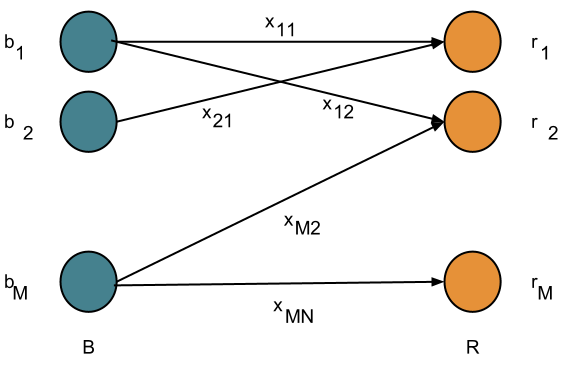
\includegraphics[width=8cm]{./parts/research/rap.png}
  \caption{A graphical view of an example solution to the Recipe Approximation 
           Problem.}
  \label{fig:rap}
  \end{center}
\end{figure}

The optimal extraction fractions are modeled as the solution to an
approximation linear program, the foundations of which were described in
\S\ref{sec:approx}. Below I describe the most straightforward formulation of 
the RAP, expanding upon the work in \cite{oliver_geniusv2:_2009}. I then
describe how additional constraints can be added to the formulation given
additional information. Finally, I describe a more abstract version that adds a
notion of agency to the problem formulation.


%% \subsubsection{Formulation}

%% The goal of this formuation is to match a set of fuel requests as closely as
possible, where proximity in this sense is defined by the $L^{1}$ norm of the
distance between a mixture attribute and a target attribute. In the following
linear program, the mixture attribute is the dot product of a matrix and a
vector. The matrix is that of all isotopic masses in barrels, $M$, where an
entry, $M_{b,i}$, is the mass of isotope $i$ in barrel $b$. The vector is the
decision variables for a given recipe, $\vec{x_{r}}$, where an entry, $x_{b,r}$,
is the fraction of barrel $b$ being assigned to fuel request $r$. The target
attribute is the target fuel request composition, $\vec{t_{r}}$. where an entry,
$t_{i,r}$, is the mass of isotope $i$ in fuel request $r$.

The minimization objective in and of itself is not necessarily interesting. In
order to enforce physical realities and domain-level knowledge, additional
constraints are added that the result must comply with. These include total
mass, isotopic masses, and neutronics constraints. I present the full
formulation below in Equation \ref{eqs:rap} and explain more fully its
derivation and interpretation in the following paragraphs.

%%% 
\begin{subequations}\label{eqs:rap}
  \begin{align}
    %%
    \min_{z} \:\: & 
    z = \sum_{r \in R} \vec{c_{r}}^{\top} \cdot \vec{y_{r}}
    & \label{eqs:rap_obj} \\
    %%
    \text{s.t.} \:\: &
    \vec{y_{r}} = \left| M \cdot \vec{x_{r}}  - \vec{t_{r}} \right|
    &
    \: \forall \: r \in R \label{eqs:rap_iso} \\
    %%
    &
    \epsilon_{m} \geq \left| \sum_{b \in B} m_{b} x_{b,r} - m_{r} \right|
    & 
    \forall \: r \in R \label{eqs:rap_mass} \\
    %%
    &
    \epsilon_{\eta} \sum_{b \in B} \eta_{b}^{-} x_{b,r} \geq 
    \left| \sum_{b \in B} \eta_{b}^{+} x_{b,r} - 
           \eta_{r} \sum_{b \in B} \eta_{b}^{-} x_{b,r} \right|
    & 
    \forall \: r \in R \label{eqs:rap_eta} \\
    &
    \sum_{r \in R} x_{b,r} \leq 1
    & 
    \forall \: b \in B \label{eqs:rap_conserv} \\
    &
    x_{b,r} \in \left[ 0, 1 \right]
    & 
    \forall \: b \in B, \forall \: r \in R  \label{eqs:rap_x}
    %%
  \end{align}
\end{subequations}
%%% 

Let me begin the discussion of the RAP formulation by noting that the
$\vec{y_{r}}$ variables occur twice, once as an assignment in
Equation \ref{eqs:rap_iso} and again in Equation \ref{eqs:rap_obj}, the
objective function. The $\vec{y_{r}}$ variables are column vectors that
represent the different between the isotopic composition of a proposed mixed
solution for a target fuel request, $r$, and the target fuel request itself. The
goal of this formulation is to minimize that difference. However, a strict
difference minimization is not directly suitable. Because separations plants can
separate materials only on elemental scales, not on isotopic scales, and because
fuel recipes are isotopic-specific, there will inevitively be isotopes present
in the barrels that are not requested in the recipe. This is described formally
in Equation \ref{eqs:barrel-req-iso}.

\begin{equation}
\label{eqs:barrel-req-iso}
I_{B} \supseteq I_{r} \: \forall r \in R
\end{equation}

Additionally, the isotopes that are most important from a nuclear engineering
domain knowledge point of view are known to of relatively low concentration in
the final fuel recipe (e.g., U-235 is only 3-5 w/o of LWR fuel). Accordingly,
some kind of weighting function is required to determine the relative importance
among isotopes in the resulting solution. I adopt Oliver's definition of this
weight from \cite{oliver_geniusv2:_2009}, which normalizes the importance of
isotopes in the final mixture.

\begin{equation}
c_{i,r} = 
\begin{cases}
 \frac{1}{m_{i,r}} & \text{if } i \in I_{r} \\
 \frac{1}{m_{r}}   & \text{if } i \not\in I_{r}
\end{cases}
\end{equation}

Note that the dot product of the vectors $\vec{y_{r}}$ and $\vec{c_{r}}^{\top}$
results in a scalar, and we wish to minimize the aggregate sum of scalars for
all fuel requests.

Moving on to the physical constraints, let us cover the simpler
Equation \ref{eqs:rap_mass} first. This constraint states that the mass of a
feasible matching solution, i.e. $\sum_{b \in B} m_{b} x_{b,r}$, must be within
some range of the mass of the given fuel request, $m_{r}$. This range is defined
by some small value, $\epsilon_{m}$. It is important to realize that the
$\epsilon$ vaules appearing in these constraints critically affect the
feasibility space. Whereas the objective function seeks to minimize the
difference between a mixture attribute and target attribute, the $\epsilon$
values define a maximum allowable difference. Accordingly, the define the bounds
of the feasible solution space. It entirely possible that during the course of a
simulation, an instance of the RAP will not have a feasible solution. In such a
scenario, the various $\epsilon$ values will have to be incrementally increased,
or relaxed, until feasibility is attained.

The neutronics constraint, Equation \ref{eqs:rap_eta}, is more complicated and
deserves its own derivation. First, note its purpose. It is a constraint on the
neutronics parameter $\eta$, i.e., the number of neutrons produced per fission
per absorption in the fuel. It is a material-specific value, which is to say
that it is a function only of material properties of the fuel, rather than the
reactor geometry or the material properties of the fuel or the moderator, as are
most other neutronics-related parameters, e.g. the effective multiplication
factor, $k_{eff}$. This parameter is ideal for an initial attempt at this
formulation because it requires only the minimal information associated with
material requests in \Cyclus, i.e., a quantity and an isotopic profile. The
equation for $\eta$ of a homogenous medium is as follows.

\begin{equation}
\label{eqs:eta_macro}
\eta = \frac{\sum_{i \in I} \nu^{i} \Sigma_{f}^{i}}
            {\sum_{i \in I} \Sigma_{a}^{i}}
\end{equation}

In Equation \ref{eqs:eta_macro}, $I$ is the set of isotopes in the material,
$\nu^{i}$ is the average neutrons produced per fisison of isotope $i$,
$\Sigma_{f}^{i}$ is the macroscopic cross section for fission of isotope $i$,
and $\Sigma_{a}^{i}$ is the macroscopic cross section for absorption of isotope
$i$. The ratio of the two cross sections produces the probability that a neutron
causes fission given that is absorbed by isotope $i$. For our purposes, because
we do not know how much of each material will contribute to a final mixture, it
is more ideal to work with microscopic cross sections and number densities of an
isotope $i$, $N^{i}$, as shown in Equation \ref{eqs:eta_micro}.

\begin{equation}
\label{eqs:eta_micro}
\eta = \frac{\sum_{i \in I} \nu^{i} \sigma_{f}^{i} N^{i}}
            {\sum_{i \in I} \sigma_{a}^{i} N^{i}}
\end{equation}

In order to discuss this in terms of barrel fractions, we must include them as
multiples of the number densities. 

\begin{equation}
\label{eqs:eta_fractions_nonlin}
\eta_{B} = \frac{\sum_{i \in I_{B}} \nu^{i} \sigma_{f}^{i} \sum_{b \in B} N_{b}^{i} x_{b}}
                {\sum_{i \in I_{B}} \sigma_{a}^{i} \sum_{b \in B} N_{b}^{i} x_{b}}
\end{equation}

In Equation \ref{eqs:eta_fractions_nonlin}, $I_{B}$ denotes the set of all
isotopes in barrels, $N_{b}^{i}$ denotes the number density of isotope $i$ in
barrel $b$, and $\eta_{B}$ is the reproduction factor resulting from the
specific values of barrel fractions $x_{b}$. If we were to leave the definition
of $\eta_{B}$ in this form, we could formulate the constraint in
Equation \ref{eqs:rap_eta} in the same way as is done in
Equation \ref{eqs:rap_mass}.

\begin{equation}
\label{eqs:eta_nonlin}
\epsilon_{\eta} \geq \left| 
\frac{\sum_{i \in I_{B}} \nu^{i} \sigma_{f}^{i} \sum_{b \in B} N_{b}^{i} x_{b,r}}
     {\sum_{i \in I_{B}} \sigma_{a}^{i} \sum_{b \in B} N_{b}^{i} x_{b,r}} 
- \eta_{r} \right|
\: \forall \: r \in R
\end{equation}

$\eta_{r}$ in Equation \ref{eqs:eta_nonlin} is defined in the normal way.

\begin{equation}
\label{eqs:eta_r}
\eta_{r} = \frac{\sum_{i \in I_{r}} \nu^{i} \Sigma_{f}^{i}}
                {\sum_{i \in I_{r}} \Sigma_{a}^{i}}
\end{equation}

Furthermore, $\eta_{r}$ is presumed to be predefined and is a constant with
respect to the RAP. Equation \ref{eqs:eta_nonlin} presents a problem; it
introduces a ratio of decision variables, which is a nonlinearity. In general,
nonlinear programs are much more difficult to solve than linear programs and
require much more exotic techniques. Some algebra can relieve this issue,
however. We begin by massaging Equation \ref{eqs:eta_nonlin}, reformulating it
into Equation \ref{eqs:eta_fractions_nonlin}.

\begin{equation}
\label{eqs:eta_fractions_lin}
\eta_{B} = \frac{\sum_{b \in B} x_{b} \sum_{i \in I_{b}} \nu^{i} \sigma_{f}^{i} N_{b}^{i}}
                {\sum_{b \in B} x_{b} \sum_{i \in I_{b}} \sigma_{a}^{i} N_{b}^{i}}
\end{equation}

Note that out of Equation \ref{eqs:eta_fractions_nonlin} fall two parameters
that are defined for each barrel, which I denote $\eta_{b}^{+}$ and
$\eta_{b}^{-}$.

\begin{equation}
\label{eqs:eta_+}
\eta_{b}^{+} \equiv \sum_{i \in I_{b}} \nu^{i} \sigma_{f}^{i} N_{b}^{i}
\end{equation}

\begin{equation}
\label{eqs:eta_-}
\eta_{b}^{-} \equiv \sum_{i \in I_{b}} \sigma_{a}^{i} N_{b}^{i}
\end{equation}

Equations \ref{eqs:eta_+} and \ref{eqs:eta_-} allow us to write
Equation \ref{eqs:eta_fractions_lin} more simply.

\begin{equation}
\label{eqs:eta_simple}
\eta_{B} = \frac{\sum_{b \in B} \eta_{b}^{+} x_{b}}
                {\sum_{b \in B} \eta_{b}^{-} x_{b}}
\end{equation}

We can then rewrite Equation \ref{eqs:eta_nonlin} using
Equation \ref{eqs:eta_simple}.

\begin{equation}
\label{eqs:eta_nonlin_simple}
\epsilon_{\eta} \geq \left| 
\frac{\sum_{b \in B} \eta_{b}^{+} x_{b_r}}
     {\sum_{b \in B} \eta_{b}^{-} x_{b_r}}
- \eta_{r} \right|
\: \forall \: r \in R
\end{equation}

Finally, we can multiply Equation \ref{eqs:eta_nonlin_simple} through by the
denominator of Equation \ref{eqs:eta_simple} to arrive at the form of the
constraint in \ref{eqs:rap_eta}.

\begin{equation}
\label{eqs:eta_linear}
\epsilon_{\eta} \sum_{b \in B} \eta_{b}^{-} x_{b,r} \geq
\left| \sum_{b \in B} \eta_{b}^{+} x_{b,r}
- \eta_{r} \sum_{b \in B} \eta_{b}^{-} x_{b,r} \right|
\: \forall \: r \in R
\end{equation}

The constraint in Equation \ref{eqs:eta_linear} has been linearized, and the
polynomial-time Simplex Method can again be applied as the solution mechanism. 

Finally, let me discuss Equations \ref{eqs:rap_conserv} and \ref{eqs:rap_x}.
Equation \ref{eqs:rap_conserv} simply states that the sum of all barrel
fractions for any given barrel must be less than one. This is simply a check on
reality -- you can't take more things from a container than exist in the
container in the first place. Equation \ref{eqs:rap_x} simply defines the notion of
a fraction, saying that all barrel fractions must lie in the range of 0 and 1,
inclusive.


%% \paragraph{Additional Constraints}

%% A viable critique of the proposal of the formulation of the RAP is that it does
not capture reactor-specific information in its application of a neutronics
parameter approximation. This initial formulation uses the neutron production
factor ($\eta$) primarily because of precedence and because of the nature of the
\Cyclus simulation engine. As it is currently designed, the \Cyclus engine
treats facilities as black boxes, which is to say that it only concerned with
material flowing into and out of those boxes for which there may or may not be
an isotopic profile accompanying an amount of requested material. This loose
coupling is by design, the \Cyclus development team wishes to maintain the
ease-of-use of connecting new simulation entities at run time, as was described
in the dynamic loading segment of \S\ref{sec:prev-dynamic}. Accordingly,
decisions to include facility-specific information, e.g. reactor assembly
characteristics, must be made with forethought and knowledge as to their
usefulness for inclusion and straining the minimal-connections model. However,
as future work progresses, such a need may arise.

One possible extension of the RAP formulation that includes reactor information
(albeit minimally) would be a use of a $k_{\infty}$ constraint either in
conjunction with or instead of the $\eta$ constraint. If used in conjunction
with the $\eta$ constraint, the new formulation would effectively add loss
information due to the presence of moderator parameters, creating a tighter
feasible solution space than would exist with simply using a $k_{\infty}$
constraint in isolation. 

The definition of $k_{\infty}$ is as follows.

\begin{equation}\label{eqs:kinf_macro}
k_{\infty} = \frac{\sum_{i \in I_{F}} \nu^{i} \Sigma_{f}^{i}}
                  {\Sigma_{a}^{M} + \sum_{i \in I_{F}} \Sigma_{a}^{i}}
\end{equation}

The notation is almost the same as Equation \ref{eqs:eta_macro}, except that the
difference between fuel and moderator cross sections are denoted by $F$ and $M$
superscripts respectively. For the remainder of this section, though, I will
drop the $F$ superscript because it can be assumed that the isotopes under
consideration for this problem are those of the fuel. The moderator-based
neutron losses are also accounted for in the denominator of the expression. It
should be noted again that this expression assumes a homogenization of fuel and
moderator material, i.e., they are considered ``smeared''. The corresponding
constraint would take the following form, again, similarly to Equation
\ref{eqs:eta_nonlin}.

\begin{equation}
\label{eqs:kinf_nonlin}
\epsilon_{k_{\infty}} \geq \left| 
\frac{\sum_{i \in I_{B}} \nu^{i} \sigma_{f}^{i} \sum_{b \in B} N_{b}^{i} x_{b,r}}
     {\Sigma_{a,r}^{M} + \sum_{i \in I_{B}} \sigma_{a}^{i} \sum_{b \in B} N_{b}^{i} x_{b,r}} 
- k_{\infty,r} \right|
\: \forall \: r \in R
\end{equation}

$k_{\infty,r}$ in Equation \ref{eqs:kinf_nonlin} is defined in the normal way.

\begin{equation}
\label{eqs:kinf_r}
k_{\infty,r} = \frac{\sum_{i \in I_{r}} \nu^{i} \Sigma_{f}^{i}}
                    {\Sigma_{a,r}^{M} + \sum_{i \in I_{r}} \Sigma_{a}^{i}}
\end{equation}

Applying similar operations to Equation \ref{eqs:kinf_nonlin} as were applied to
Equation \ref{eqs:eta_nonlin} result in a similarly linearized constraint.

\begin{equation}
\label{eqs:kinf_linear}
\epsilon_{k_{\infty}} \left( \Sigma_{a,r}^{M} + \sum_{b \in B} \eta_{b}^{-} x_{b,r} \right)
\geq
\left| \sum_{b \in B} \eta_{b}^{+} x_{b,r}
- k_{\infty,r}  \left( \Sigma_{a,r}^{M} + \sum_{b \in B} \eta_{b}^{-} x_{b,r} \right) \right|
\: \forall \: r \in R
\end{equation}

As can be seen, increasing the information in given to the problem formulation
increases the complexity of the formulation. Further, to preserve the linear
nature of the formulation, any additional parameters that we wish to provide a
constraint for must be able to be decomposed into, at worst, a ratio of linear
combinations of barrel-specific parameters and barrel fractions. Should this
formulation prove too simplistic in practice, one way forward would be to move
into the nonlinear realm of approximation formulations. This would open up a
much more robust set of parameters that we could constrain and would also allow
usage of tighter norms than the $L_1$ norm, e.g. the $L_2$ norm. However,
solution techniques for nonlinear programs are significantly more complicated
and computationally time consuming than for linear programs. Indeed, they
constitute an entirely new field of study.


%% \paragraph{Agency and Abstraction}

%% In the previous sections, we have assumed a fundamental truth in our formulation
of the RAP: reactors requesting nuclear fuel know exactly what isotopes they
want and in what quantities they want them. This notion has merit in general; in
real life, the companies that manage reactors and their fuel do, in fact, know
the exact specifications of fuel they want. However, this knowledge comes from
two sources: the availability of the fuel they can purchase at some cost and a
thorough analysis of the effect of various fuels to their reactor flux profiles
and thus their ability to reach high levels of burnup, or fuel
utilization. Furthermore, simulators to date that allow for isotopic-level
dependence of input and output fuel have relied almost solely on the notion of
recipes, hence it made sense when the original RAP formulation was conceived to
have the objective function minimize the $L_1$ norm of the isotopic
vector. Additionally, this is a viable first step that has yet to be shown in
any sort of proof-of-principle, as this work proposes to do.

The original goal of developing such a separations/fuel fabrication facility
that interacts in a fuel cycle simulation is to provide a semblance of realism
with respect to the global inventory of separated material for reactors that
want fuel made out of such material. Critically, this semblance of realism is
\textit{automated} along the similar lines of Scopatz's work for
reactors~\cite{scopatz_essential_2011} and Huff's work for
repositories~\cite{huff_integrated_2013}. Accordingly, the notion that reactors
must know \textit{a priori} the exact fuel recipe they require at any given time
step is, at best, a large approximation. Something that is perhaps closer to
reality is to allow reactors to determine its most important parameter, whether
or not it is in fact an exact fuel recipe. For example, it is a viable
possibility that a reactor would take any reprocessed fuel type that fits
certain parameters, such as a beginning-of-cycle reactivity and a maximum void
coefficient of reactivity. The former parameter is a measure of fuel
utilization, i.e., how long fuel can stay in a reactor before becoming a net
neutron poison, and the latter is a measure of reactor criticality
safety. Accordingly, such a recipe order would effectively connote a notion of
requiring a minimum fuel utilization while maintaining certain safety
parameters, both of which are functions of the resulting isotopics of the given
solution, but neither of which demand specific levels of isotopics.

The RAP formulation can be extended to allow such a level of abstraction with
respect to its objective function and constraints. Let me note beforehand that
this proposed change, while introducing increased agency into the simulation
(allowing reactors greater autonomy over decision-making processes), it
increases connectivity between specific types of facilities, the proposed
separations facility and reactors in this case. Again, \Cyclus has been designed
to minimize these facility-specific connections, so adding them must be done
with sufficient knowledge as to their usefulness. In any case, the point of this
section is to simply show the extension required to the RAP in order to achieve
this aim mathematically.

Let us assume that we have at our disposal the three parameters used in Equation
\ref{eqs:rap}, namely the $L_1$ norm of the isotopic vector, the total mass, and
$\eta$, the neutron production factor. Further, let us assume that there are
three sets of reactors ordering fuel, corresponding to each parameter. I will
denote them as $R_I$, $R_m$, and $R_\eta$ respectively. 

It is important to reiterate the nature of the approximation problem before
continuing, because we are modifying it from its original purpose. As described
in \S\ref{sec:approx}, the approximation problem is concerned with finding an
approximate solution vector, $\vec{x}$, that gets ``close'' to a correct
solution to the matrix equation, i.e., 

\begin{equation*}
  \mathbf{A} \vec{x} \approx \vec{b}.
\end{equation*}

The RAP then applies a weighting coefficient in the objective function due to
domain knowledge of the problem, whereas the unit vector, $\vec{e}$, is used in
the original approximation formulation. The use of the $L_1$ norm is appropriate
in the original RAP case because the mass of isotopes is being approximated,
which is an extrinsic quantity specific to each isotope in the set of
isotopes. Accordingly, such a powerful technique is not required if one is
approximating an aggregate quantity such as overall mass or the neutron
production factor. The simplified equation for mass approximation is

\begin{equation*}
  \sum_{b \in B} m_{b} x_{b,r} \approx m_{r},
\end{equation*}

and the simplified equation for neutron production factor approximation is

\begin{equation*}
\frac{\sum_{b \in B} \eta_{b}^{+} x_{b,r}}
     {\sum_{b \in B} \eta_{b}^{-} x_{b,r}} 
\approx \eta_{r}.
\end{equation*}

We want the difference between each parameter to be approximately zero, i.e.,

\begin{equation*}
  \sum_{b \in B} m_{b} x_{b,r} - m_{r} \approx 0, \mbox{and}
\end{equation*}

\begin{equation*}
\frac{\sum_{b \in B} \eta_{b}^{+} x_{b,r}}
     {\sum_{b \in B} \eta_{b}^{-} x_{b,r}} 
- \eta_{r} \approx 0.
\end{equation*}

Accordingly, we can denote their differences as $y_{m}$ and $y_{\eta}$ and use
these values in our minimal objective function. Take special note that we want
to minimize each $y$, i.e., get them as close to zero as possible. This allows
us to again linearize the neutronics function.

\begin{equation}\label{eqs:mass_obj}
y_{m} = \left|  \sum_{b \in B} m_{b} x_{b,r} - m_{r} \right|
\end{equation}

\begin{equation}\label{eqs:eta_obj}
y_{\eta} = \left| \sum_{b \in B} \eta_{b}^{+} x_{b,r}
- \eta_{r} \sum_{b \in B} \eta_{b}^{-} x_{b,r} \right|
\end{equation}

With the additions to the objective function in hand, the RAP can then be
adapted to a slightly different formulation. Let us call this new problem the
Reactor Order Approximation Problem (ROAP). Note that it has effectively
sectioned the original RAP into three separate request spaces, applying an
objective function and constraints specific to each. Each request space is
connected by the overarching set of barrels, i.e., material must be picked from
all barrels simultaneously.

%%% 
\begin{subequations}\label{eqs:roap}
  \begin{align}
    %%
    \min_{z} \:\: & 
    z = \sum_{r \in R_I} \vec{c_{r}}^{\top} \cdot \vec{y_{I,r}}
    + \sum_{r \in R_m} y_{m,r} + \sum_{r \in R_\eta} y_{\eta,r}
    & \label{eqs:roap_obj} \\
    %%
    \text{s.t.} \:\: &
    \vec{y_{I,r}} = \left| M \cdot \vec{x_{r}}  - \vec{t_{r}} \right|
    &
    \: \forall \: r \in R_I \label{eqs:roap_iso_y} \\
    %%
    &
    y_{m,r} = \left| \sum_{b \in B} m_{b} x_{b,r} - m_{r} \right| 
    &
    \: \forall \: r \in R_m \label{eqs:roap_mass_y} \\
    %%
    &
    y_{\eta} = \left| \sum_{b \in B} \eta_{b}^{+} x_{b,r}
    - \eta_{r} \sum_{b \in B} \eta_{b}^{-} x_{b,r} \right|
    &
    \: \forall \: r \in R_\eta \label{eqs:roap_eta_y} \\
    %%
    &
    \epsilon_{m} \geq \left| \sum_{b \in B} m_{b} x_{b,r} - m_{r} \right|
    & 
    \forall \: r \in R_m, \: \forall \: r \in R_{\eta} \label{eqs:roap_mass} \\
    %%
    &
    \epsilon_{\eta} \sum_{b \in B} \eta_{b}^{-} x_{b,r} \geq 
    & \nonumber \\ 
    & 
    \:\:\:\:\:\:\:\:\:\:\:  % u-g-l-y you ain't got no alibi, you can't format =(
    \left| \sum_{b \in B} \eta_{b}^{+} x_{b,r} - 
    \eta_{r} \sum_{b \in B} \eta_{b}^{-} x_{b,r} \right|
    &
    \forall \: r \in R_{I}, \: \forall \: r \in R_{m} \label{eqs:roap_eta} \\
    %%
    &
    \sum_{r \in R_{I}} x_{b,r} +
    \sum_{r \in R_{m}} x_{b,r} + 
    \sum_{r \in R_{\eta}} x_{b,r} \leq 1
    & 
    \forall \: b \in B \label{eqs:roap_conserv} \\
    %%
    &
    x_{b,r} \in \left[ 0, 1 \right]
    & 
    \forall \: b \in B, 
    \forall \: r \in R  \label{eqs:roap_x}
    %%
  \end{align}
\end{subequations}
%%% 

where $R$ is simply the superset of the partitioned requests

\begin{equation*}
  R = R_{I} \cup R_{m} \cup R_{\eta}.
\end{equation*}


%\subsubsection{Initial Results and Benchmarks}


%% %%%%%% conclusions %%%%%%%%%%
%% \section{Results \& Conclusions}\label{sec:conclusions}
%% Presented herein are a number of simple simulations in order to 
demonstrate the capability of an implementation of the framework. We 
discuss various modeling tradeoffs encountered while constructing 
once-through and recycle simulation cases. We finish with a 
discussion of the future simulation landscape and expansion of the 
use of the framework.


%%%%%% acks %%%%%%%%%%
\section{Acknowledgments}
This research is being performed using funding received from the DOE
Office of Nuclear Energy's Nuclear Energy University Programs.  The
author thanks the NEUP for its generous support.

\includegraphics[width=1.5in]{neup_logo_large.jpg}

%%%%%% bib %%%%%%%%%%
\bibliography{./bibs/refs,./bibs/simulators,./bibs/benchmarks,./bibs/cosi,./bibs/abm-supply-chain,./bibs/blending.bib}

\end{document}
%%%%%%%%%%%%%%%%%%%%%%%%%%%%%%%%%%%%%%%%%%%%%%%%
%%%%%%%%%%%%%%%%%%%%%%%%%%%%%%%%%%%%%%%%%%%%%%%%%%%%%%%%%%%%%%%%%%%%%%%%%%%%%%%%
